% ONLY IN CHAPTER 1

\addtocontents{toc}{\vspace{2em}} % Add a gap in the contents, for aesthetics

% Begin numeric (1,2,3...) page numbering

\pagestyle{fancy} % Return the page headers back to the "fancy" style

% Chapter 1

\chapter{Introduction} % Main chapter title

\label{chap:ntroduction} % For referencing the chapter elsewhere, use \ref{Chapter1} 

\lhead{Chapter 1. \emph{Introduction}} % This is for the header on each page - perhaps a shortened title

%----------------------------------------------------------------------------------------

\section{Background and Definitions}

Graph Signal Processing (GSP) is a rapidly evolving field that sits at the intersection between spectral graph theory, statistics and data science \citep{Shuman2013}. In this context, a graph is an abstract collection of objects in which any pair may be, in some sense, ``related". These objects are referred to as vertices (or nodes) and their connections as edges \citep{Newman2018}. GSP is concerned with the mathematical analysis of signals that are defined over the nodes of a graph, referred to simply as \textit{graph signals}. 

A graph signal can be thought of as a value that is measured simultaneously at each node in a graph. In practice, it is represented as a vector where each element corresponds to a single node. For example, consider a social network where each node represents an individual and presence of an edge between two nodes indicates that the two individuals have met. An example of a graph signal in this context could be the age of each person in the network. Figure \ref{fig:graph_signal} shows a graphical depiction of a  signal defined over a network. 
  


\begin{figure}[htbp]
	\centering
		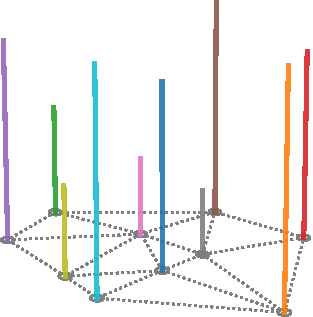
\includegraphics[width=0.4\linewidth]{Figures/graph_signal_cropped.pdf}
		\rule{35em}{0.5pt}
	\caption{A graphical depiction of a graph signal. Here, the nodes are represented by circles, the edges as dotted lines, and the value of the signal at each node is represented by the height of its associated bar. }
	\label{fig:graph_signal}
\end{figure}


Graphs and graph signals have proven a useful way to describe data across a broad range of applications owing to their flexibility and relative simplicity. They are able to summarise the of properties large, complex systems within a single easily-digestible structure. Much of the data 


The GSP community, in particular, is focused on generalising tools designed for traditional signal processing tasks to irregular graph-structured domains. 

\citep{Ortega2018}



\section{Thesis overview}